\documentclass[a4paper, oneside]{memoir}
\usepackage[utf8]{inputenc}
\usepackage[T1]{fontenc}
\usepackage{pifont}
\usepackage{amssymb}
\usepackage{fourier}
\usepackage[dvipsnames]{xcolor}
\usepackage{tikz}
\usepackage{pdfpages}
\usepackage[sfdefault]{roboto}
\usepackage{color}

% Styles
\tikzstyle{teamshare} = [below, text width=5.4cm, inner sep = 0.5cm, text=white, align=center]
\tikzstyle{cardtext} = [below, text width=5.9cm, inner sep = 0.25cm, text centered]
\setlrmarginsandblock{0.9cm}{*}{1}
\setulmarginsandblock{1.49cm}{*}{1}
\checkandfixthelayout[nearest]
\pagestyle{empty}

% Define Commands
\newcommand{\condition}[1]{\textbf{#1}}
\newcommand{\character}[1]{\textbf{#1}}
\newdimen\titlespacing
\titlespacing=0.15cm

% Define Seperators
\newcommand{\seperator}[1]{\\ \vspace{\titlespacing} \hrulefill {} \tiny \bfseries #1 \normalfont \normalsize \hrulefill \\ \vspace{\titlespacing}}
\newcommand{\seperatoraction}{\seperator{POWER}}
\newcommand{\seperatordescription}{\seperator{DESCRIPTION}}
\newcommand{\seperatorcondition}{\seperator{CONDITION}}
\newcommand{\seperatorwin}{\seperator{HOW TO WIN}}
\newcommand{\redwinsection}{
	\seperatorwin
	You win if \character{Santa} does not gain the \condition{humbug} condition due to the \character{Grinch} stealing Christmas.
}
\newcommand{\greenwinsection}{
	\seperatorwin
	\small You win if \character{Santa} gains the \condition{humbug} condition due to the \character{Grinch} stealing Christmas.
}
\newcommand{\titlefrom}[1]{\\ \tiny > from #1 <\normalsize}

% Begin Document
\begin{document}
	
% New Page
\noindent 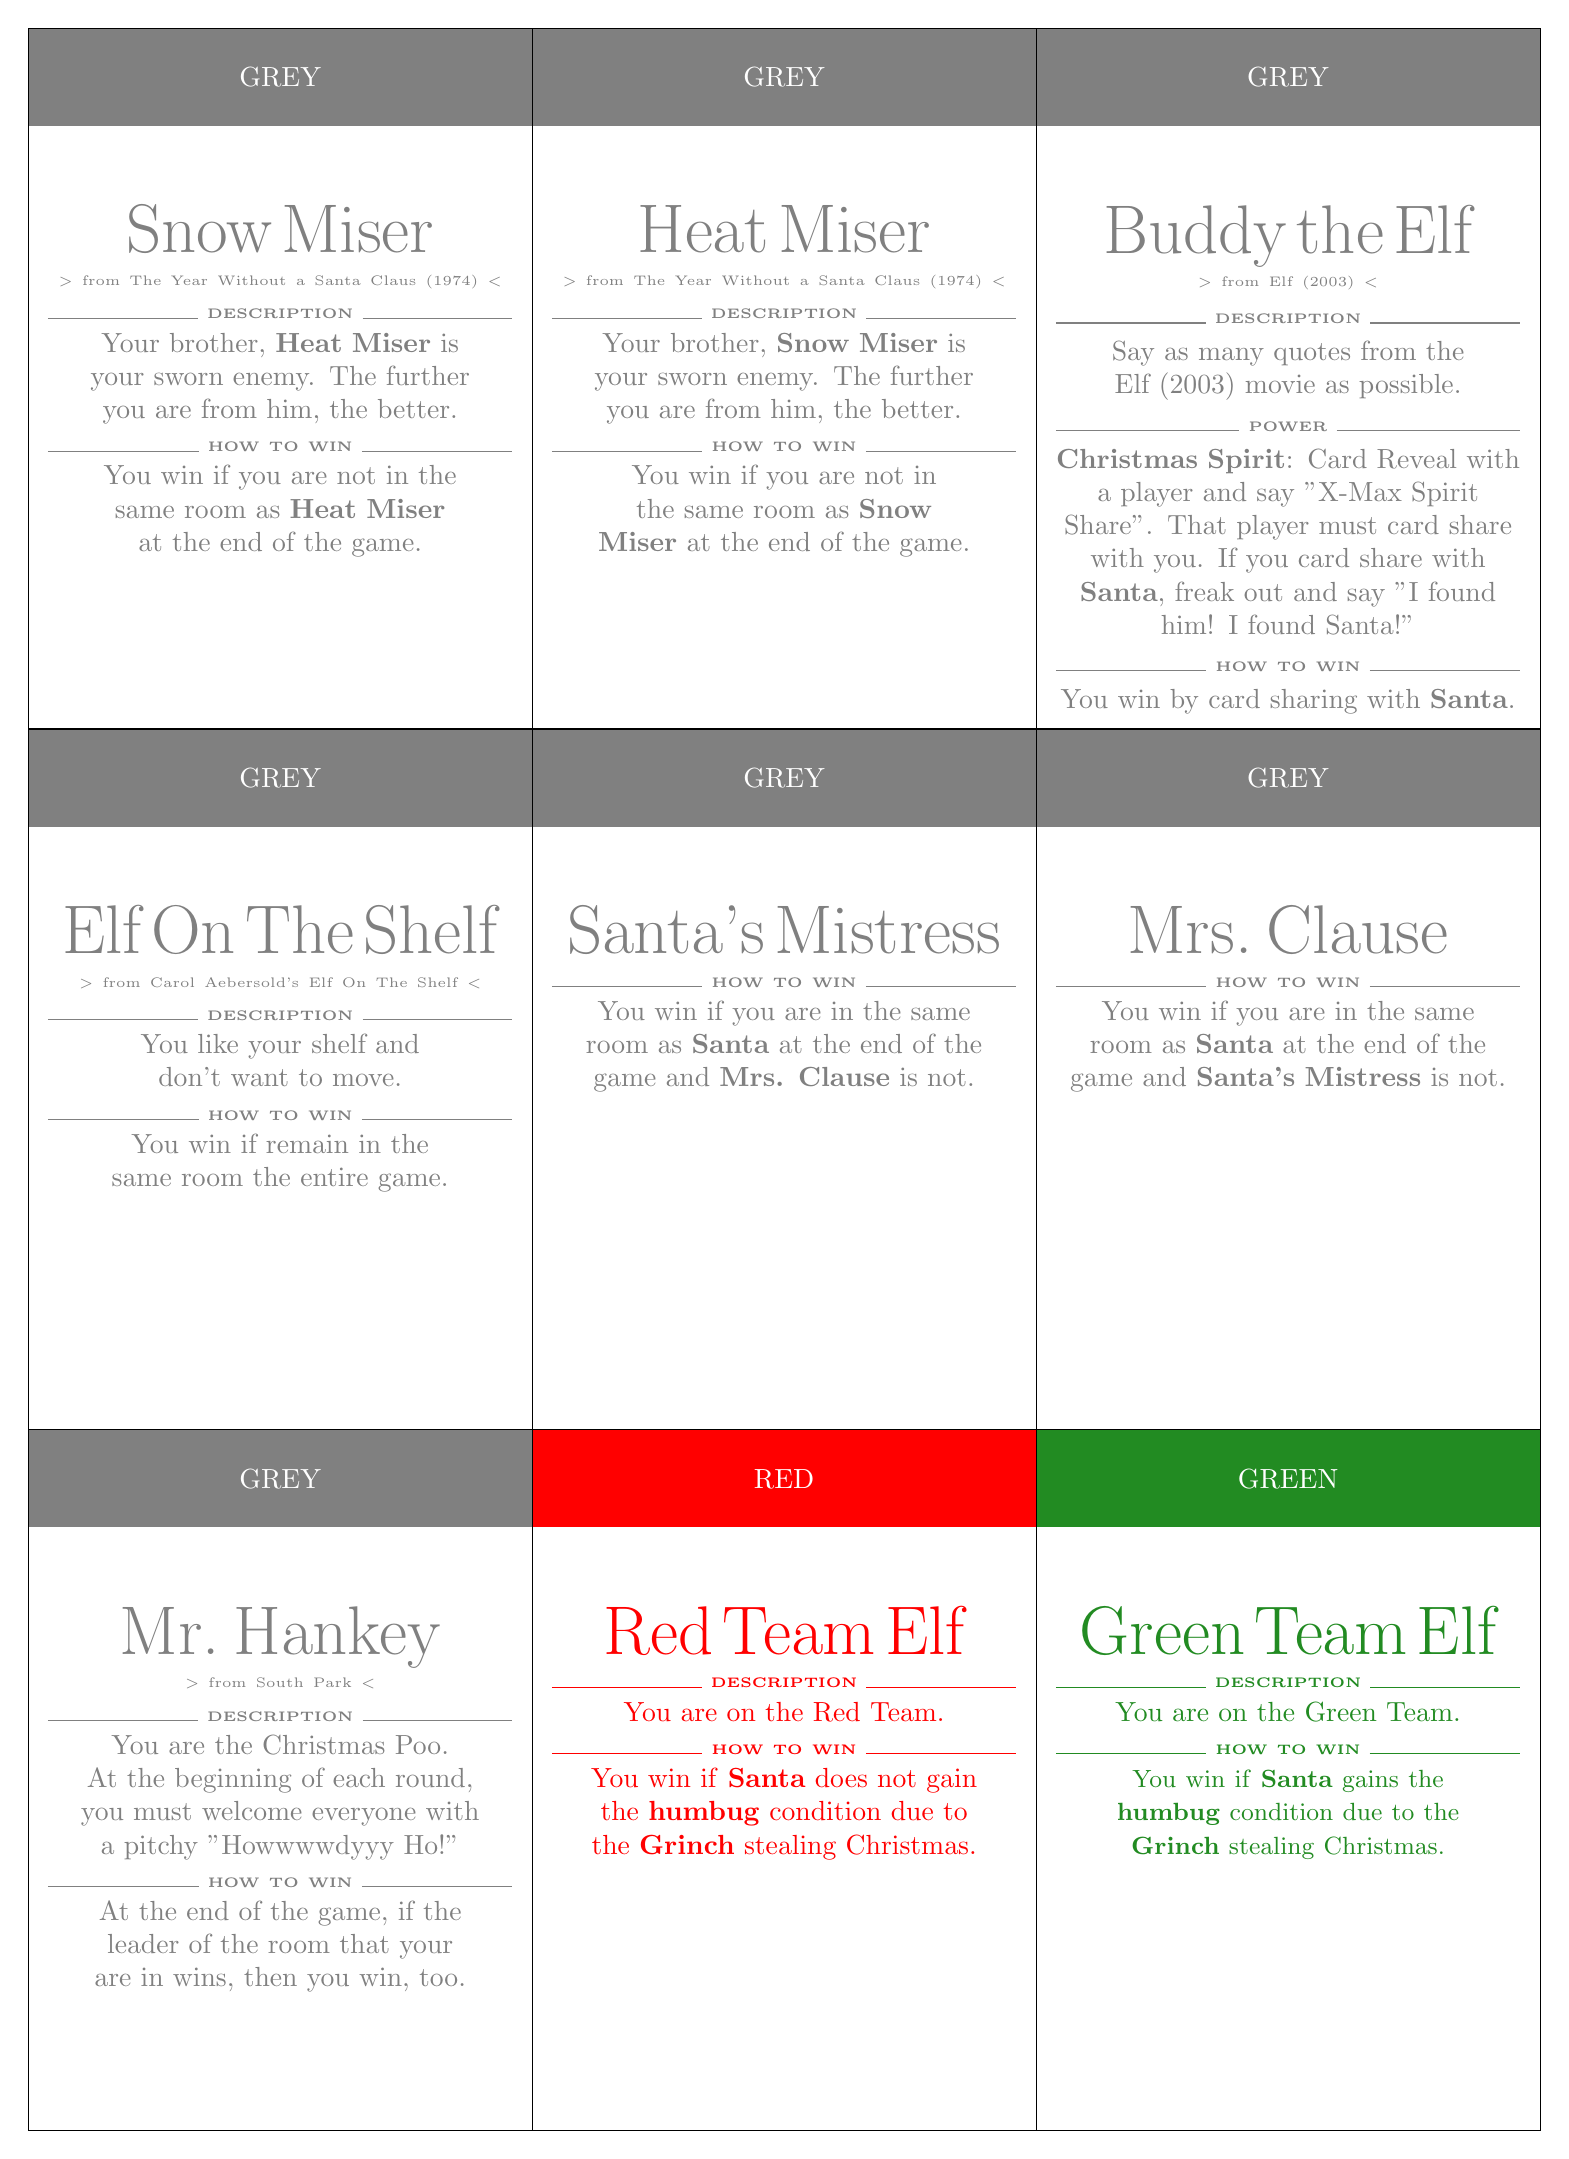
\begin{tikzpicture}[outer sep=0]

% SNOW MISER
\node[teamshare, fill=gray] (1) at (3.2,26.7) {\HUGE GREY};
\node[cardtext, text=gray] at (3.2,24.7) {
	{\Huge Snow Miser}
	\titlefrom{The Year Without a Santa Claus (1974)}
	\seperatordescription
	Your brother, \character{Heat Miser} is your sworn enemy. The further you are from him, the better.
	\seperatorwin
	You win if you are not in the same room as \character{Heat Miser} at the end of the game.
};

% HEAT MISER
\node[teamshare, fill=gray] at (9.6,26.7) {\HUGE GREY};
\node[cardtext, text=gray] at (9.6,24.7) {
	{\Huge Heat Miser}
	\titlefrom{The Year Without a Santa Claus (1974)}
	\seperatordescription
	Your brother, \character{Snow Miser} is your sworn enemy. The further you are from him, the better.
	\seperatorwin
	You win if you are not in the same room as \character{Snow Miser} at the end of the game.
};

% BUDDY THE ELF
\node[teamshare, fill=gray] at (16,26.7) {\HUGE GREY};
\node[cardtext, text=gray] at (16,24.7) {
	\titlespacing=.05cm
	{\Huge Buddy the Elf}
	\titlefrom{Elf (2003)}
	\seperatordescription
	Say as many quotes from the Elf (2003) movie as possible.
	\seperatoraction
	\condition{Christmas Spirit}: Card Reveal with \\
	a player and say "X-Max Spirit \\
	Share". That player must card share \\
	with you. If you card share with \\
	\condition{Santa}, freak out and say "I found \\
	him! I found Santa!"
	\seperatorwin
	You win by card sharing with \condition{Santa}.
	\titlespacing=0.15cm
};

% ELF ON THE SHELF
\node[teamshare, fill=gray] at (3.2,17.8) {\HUGE GREY};
\node[cardtext, text=gray] at (3.2,15.8) {
	{\Huge Elf On The Shelf}
	\titlefrom{Carol Aebersold's Elf  On The Shelf}
	\seperatordescription
	You like your shelf and don't want to move.
	\seperatorwin
	You win if remain in the same room the entire game.
};

% SANTA'S MISTRESS
\node[teamshare, fill=gray] at (9.6,17.8) {\HUGE GREY};
\node[cardtext, text=gray] at (9.6,15.8) {
	{\Huge Santa's Mistress}
	\seperatorwin
	You win if you are in the same room as \condition{Santa} at the end of the game and \condition{Mrs. Clause} is not.
};

% MRS. CLAUSE
\node[teamshare, fill=gray] at (16,17.8) {\HUGE GREY};
\node[cardtext, text=gray] at (16,15.8) {
	{\Huge Mrs. Clause}
	\seperatorwin
	You win if you are in the same room as \condition{Santa} at the end of the game and \condition{Santa's Mistress} is not.
};

% MR. HANKEY, THE CHRISTMAS POO
\node[teamshare, fill=gray] at (3.2,8.9) {\HUGE GREY};
\node[cardtext, text=gray] at (3.2,6.9) {
	{\Huge Mr. Hankey}
	\titlefrom{South Park}
	\seperatordescription
	You are the Christmas Poo. \\At the beginning of each round, you must welcome everyone with a pitchy "Howwwwdyyy Ho!"
	\seperatorwin
	At the end of the game, if the leader of the room that your are in wins, then you win, too.
};

% RED TEAM ELF
\node[teamshare, fill=red] at (9.6,8.9) {\HUGE RED};
\node[cardtext, text=red] at (9.6,6.9) {
	{\Huge Red Team Elf}
	\seperatordescription
	You are on the Red Team.
	\redwinsection
};

% GREEN TEAM ELF
\node[teamshare, fill=ForestGreen] at (16,8.9) {\HUGE GREEN};
\node[cardtext, text=ForestGreen] at (16,6.9) {
	{\Huge Green Team Elf}
	\seperatordescription
	You are on the Green Team.
	\greenwinsection
};


\draw (0,0) -- (19.2,0);
\draw (0,8.9) -- (19.2,8.9);
\draw (0,17.8) -- (19.2,17.8);
\draw (0,26.7) -- (19.2,26.7);

\draw (0,0) -- (0,26.7);
\draw (6.4,0) -- (6.4,26.7);
\draw (12.8,0) -- (12.8,26.7);
\draw (19.2,0) -- (19.2,26.7);



\end{tikzpicture}

%Background is not my own. But courtesy of a user on BGG
\includepdf[pages={1}, angle=90]{cardsbackground.pdf}




\end{document}